\documentclass[a4paper, 12pt]{article}
 
\usepackage[applemac]{inputenc}
\usepackage{graphicx}
\usepackage[french]{babel}
\usepackage[T1]{fontenc}
\usepackage{lmodern}
\usepackage{float}
%\usepackage{fullpage}


 
\begin{document}
 
\title{TL Programming Assignment 3}
\author{Mathurin \textsc{Massias} \and Cl�ment \textsc{Nicolle}}
\date{\today} 
 
\maketitle

\section{Full information, partial information}
\hspace{-6mm}\textbf{1):} It is a problem with full information since $R_A$ is known by $A$. A problem with partial information would be %TODO


\section{EWF and EXP3 versus an oblivious adversary}
\underline{Question 1:} We choose as a sequence for $B$ : $(1, 2, 2, 1, 2, 2, 1, \ldots)$ 
\\[3mm]We take $\eta = \sqrt{\frac{N \mathrm{log} N}{n(e-1)}}$ (formula from the class, here $N = 2$) and $\eta = 0.04$. For EXP3 we also take $\beta = \eta$.
\\We get the following regret curves :


\begin{figure}[H]
\centering
\noindent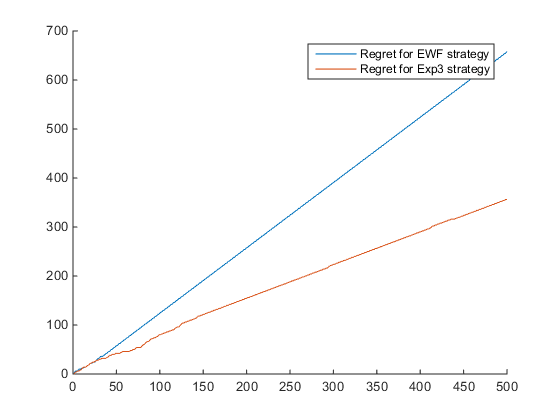
\includegraphics[scale=0.7]{Q1-regrets.png}
\caption{Regrets for EXP3 and EWF strategy}
\end{figure}



\section{EXP3 versus EXP3 : Nash Equilibrium}
\textbf{2):} 

\begin{figure}[H]
\centering
\noindent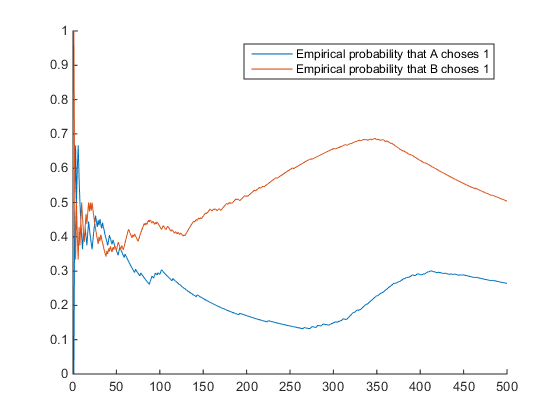
\includegraphics[scale=0.7]{Q2-probas.png}
\caption{Convergence of empirical probabilities at horizon 500}
\end{figure}

\underline{Question 2}

\begin{figure}[H]
\centering
\noindent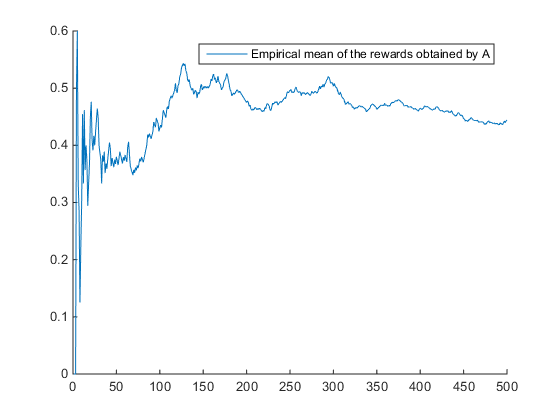
\includegraphics[scale=0.7]{Q2-rewards.png}
\caption{Convergence of the mean reward for player A}
\end{figure}






\end{document}